\section{Fast R-CNN} \label{sec:fast_rcnn}

The author of R-CNN later implemented Fast R-CNN to reduce the runtime and space complexity while improving detection accuracy. Fast R-CNN is implemented in Python and C++. Like the R-CNN model, Fast R-CNN can be used along with any convolutional neural network. In the proposal Fast R-CNN model, the author utilized VGG16, one of the deepest CNN in 2015, as the backbone CNN for the model. Comparing the performance of Fast R-CNN with VGG16 versus R-CNN with VGG16 on the PASCAL VOC 2012 dataset while having the same setup, the experiment showed that Fast R-CNN is 9 times faster at train-time and 213 times faster at test-time while achieving a higher mAP score \cite{fast_rcnn_og}. In the next section, we will mention the keynote of VGG16 architecture, followed by the discussion of the Fast R-CNN model and its design decisions that lead to a higher mAP.

\begin{figure}[!ht]
    \centering
    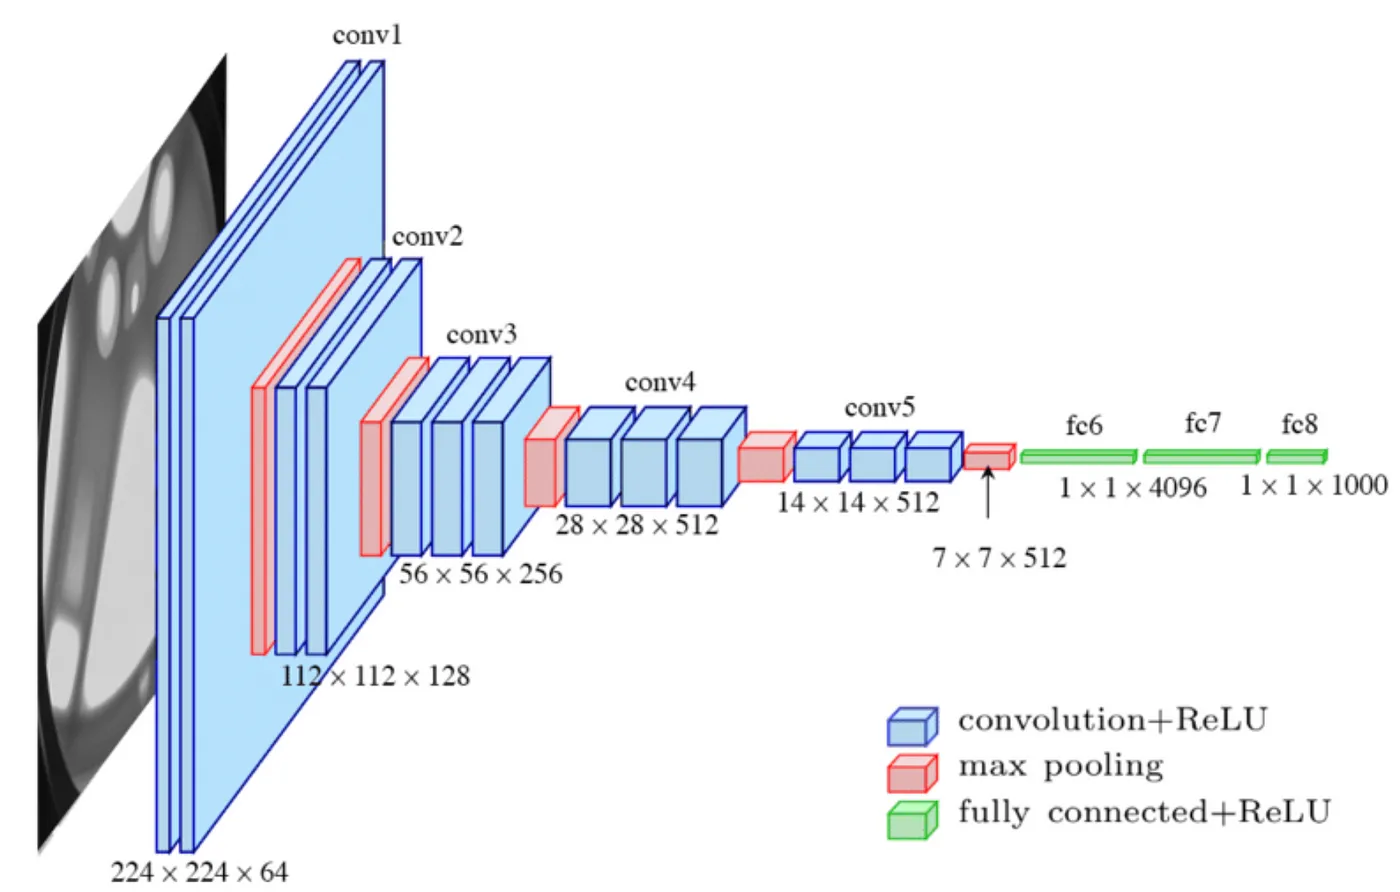
\includegraphics[width=4in]{figures/vgg16_architect.png}
    \caption{VGG16 architecture \cite{vgg16_architect_2014}}
    \label{fig:vgg16_archite}
\end{figure}

The VGG16 is a CNN model developed by the Visual Geometry Group (VGG) at the University of Oxford in 2014 \cite{vgg16_2014}. The VGG16 architecture is notably deeper than AlexNet, comprising 16 learnable layers -- 13 convolutional layers and 3 fully connected layers -- and 5 non-trainable max-pooling layers [Fig. \ref{fig:vgg16_archite}]. VGG16 takes an RGB $224 \times 224$ image as input and generates a $7 \times 7$ feature map, downsampled by a factor of 32 from the input image resolution \cite{deconv_rcnn_2018}. A set of fully connected layers is then processed in this feature map to produce the predicted classification label for the image. Unlike AlexNet, which uses a combination of $3 \times 3$ and $5 \times 5$ filters, VGG16 uses only $3 \times 3$ filters throughout the network with smaller strides and padding. By employing a strategy like utilizing a pair of stacked $3 \times 3$ layers in place of a single $5 \times 5$ layer, VGG16's design enabled it to demonstrate that elevating the depth of a network to 16 layers can yield substantial improvements for existing CNNs. Fast R-CNN adapts any CNN model for object detection by performing three changes. The first change is replacing the last pooling layer with an RoI pooling layer (named RoIPool). For VGG16, an RoI will be used in place of the $7 \times 7 \times 512$ max-pool layer in Fast R-CNN. The second change is replacing the last fully connected layer with two sibling layers, i.e., replacing the fc8 layer for VGG16. Lastly, Fast R-CNN will adjust the input layer of the CNN model to accept images of any size and proposed RoIs for that particular image as input. We will discuss these changes in more detail later in this section.

\begin{figure}[!ht]
    \centering
    \subfloat[][Overall architecture \cite{fast_rcnn_og}]{ 
        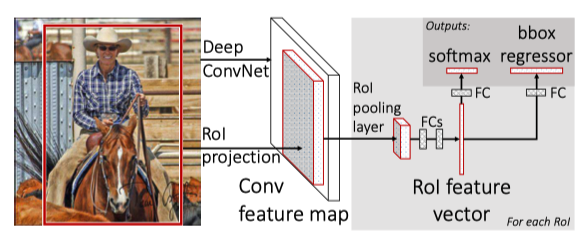
\includegraphics[width=3in]{figures/fast_rcnn_archiet.png} \label{fig:fast_rcnn_archite} 
    }

    \subfloat[][Network flow \cite{rcnn_vari_flow_chart}]{ 
        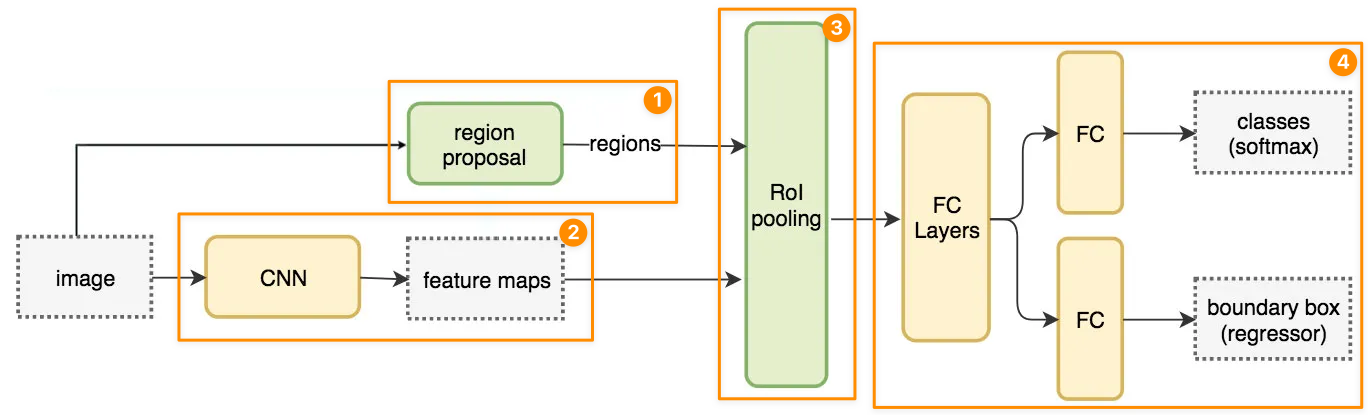
\includegraphics[width=5.5in]{figures/fast_rcnn_flowc.png} \label{fig:fast_rcnn_flowc} 
    }
    \caption{Fast R-CNN overall architecture and network flow} \label{fig:fast_rcnn_archite_flowc}
\end{figure}

The overall architecture of Fast R-CNN can be thought of as four stages [Fig. \ref{fig:fast_rcnn_archite_flowc}]. The network takes an image and a set of RoI as inputs. Comparing Fast R-CNN with R-CNN, which takes an image as an input and then generates RoIs with selective search, the type of input data between the two models is not equivalent. Thus we assume Fast R-CNN takes an image as input and performs the selective search algorithm as the first stage of the model. In the second stage, Fast R-CNN generates a feature map for the entire image by running the input image through a CNN. The CNN used for Fast R-CNN performance measurement in the original paper is VGG16. In the third stage, the model uses RoIPool layer to extract the feature grid corresponding to the proposed RoI from the image feature map generated in stage two for each proposed RoI. The RoIPool layer is also used for downsampling the RoI feature grid of any size to a pre-defined fixed-length feature vector. In the fourth stage, each RoI feature vector is processed by multiple fully connected layers and then branched into the two sibling output layers -- softmax classification and bounding box regression. The model's learning with two output branches is possible with the use of multi-task loss.

\begin{figure}[!ht]
    \centering
    \subfloat[][R-CNN architecture with stages]{ 
        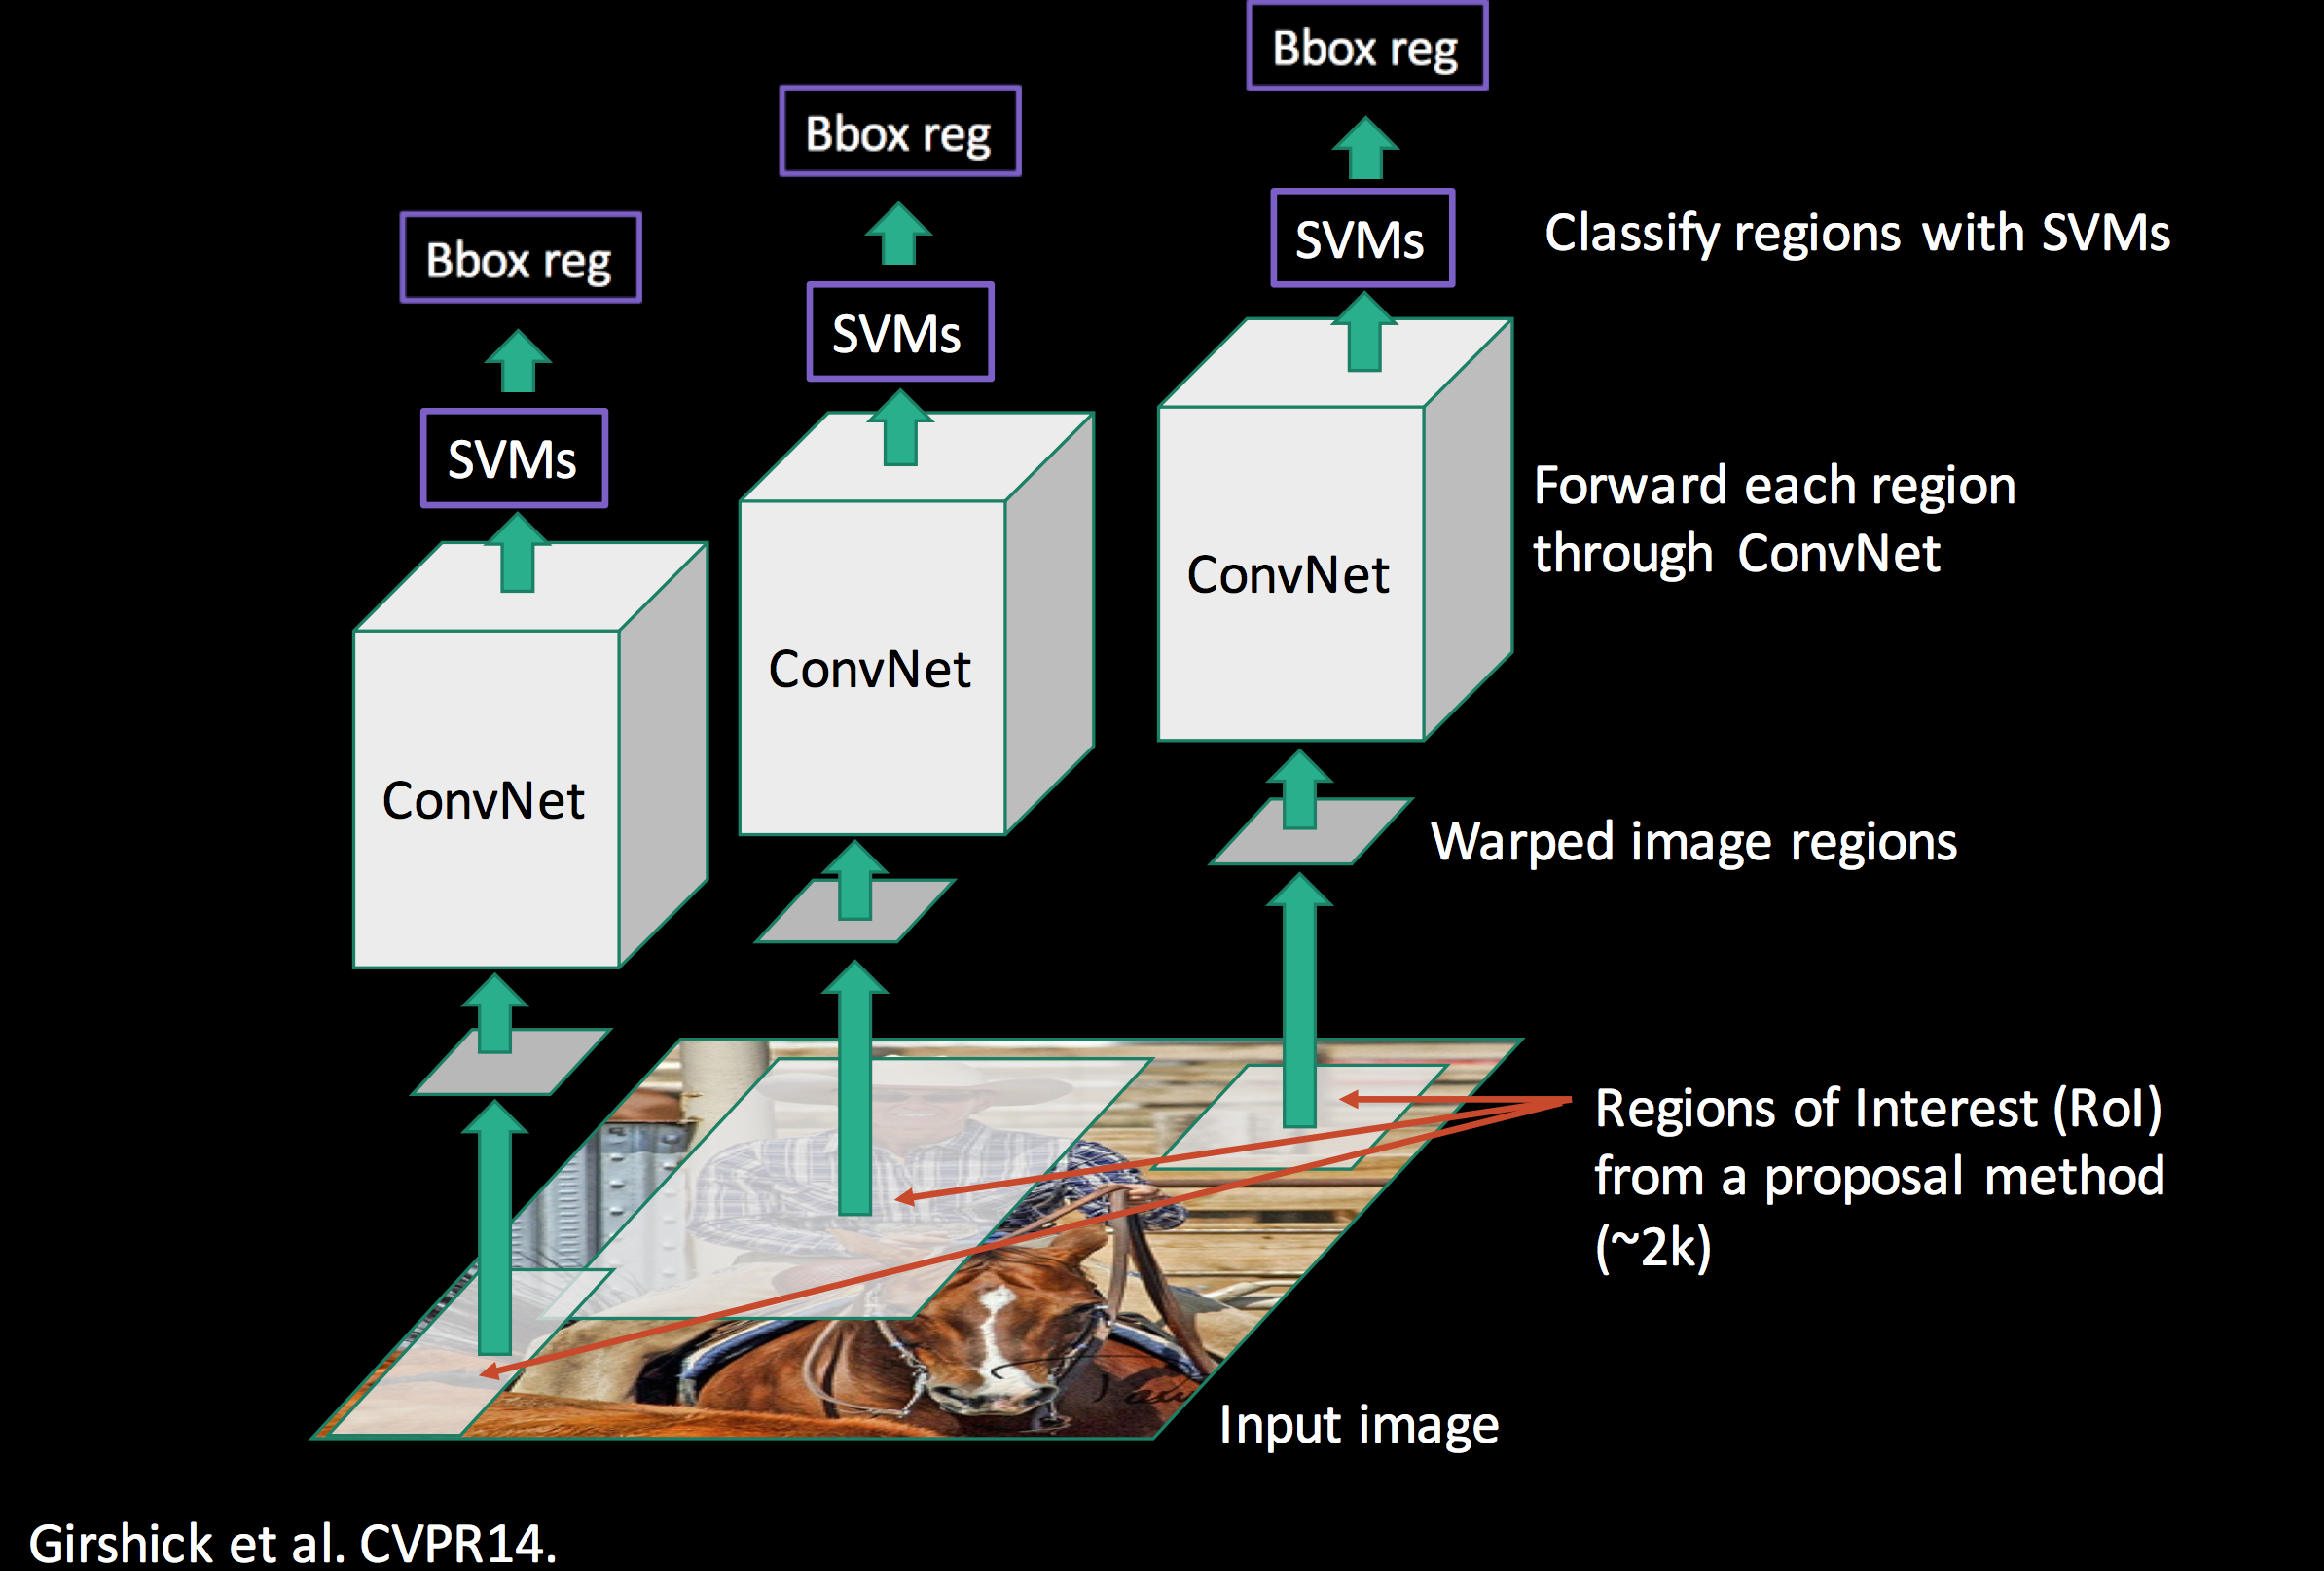
\includegraphics[height=2in]{figures/rcnn_custom_draw.png} \label{fig:rcnn_custom_draw} 
    }
    \subfloat[][Fast R-CNN architecture with stages]{ 
        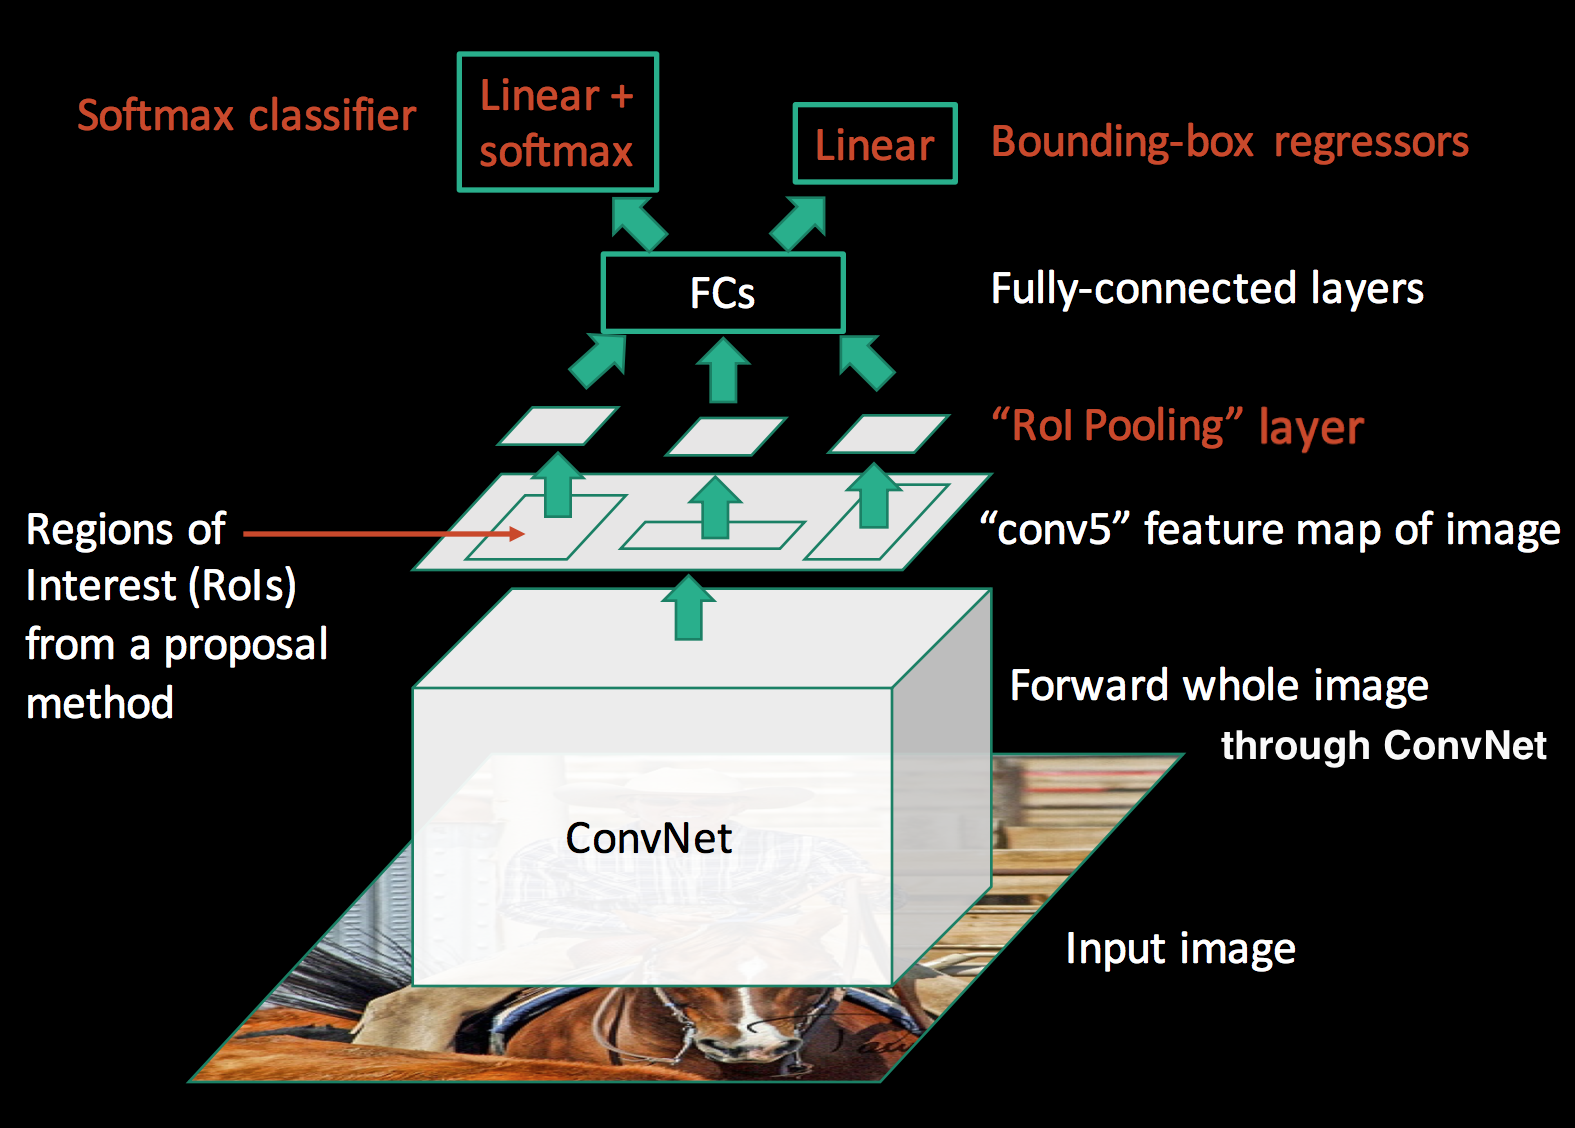
\includegraphics[height=2in]{figures/fast_rcnn_custom_draw.png} \label{fig:fast_rcnn_custom_draw} 
    }
    \caption{R-CNN vs. Fast R-CNN architecture comparison \cite{rcnn_vs_faster_custom_fig}} \label{fig:rcnn_vs_fast}
\end{figure}

Comparing the architecture of R-CNN and Fast R-CNN, there are three main differences between the two models [Fig. \ref{fig:rcnn_vs_fast}]. The first difference is that Fast R-CNN generates the feature map for the entire input image instead of each RoI individually. This means Fast R-CNN only applies CNN to image one and shares the feature maps across RoIs. Fast R-CNN behavior holds several advantages compared to treating RoIs individually, like in the R-CNN model. These advantages are reducing the use of disk storage, reducing redundancy operation performed on overlapping RoI, and sharing computation power and memory used between RoIs in the same image, thus improving the performance at test-time \cite{fast_rcnn_og}. Sharing the feature map and memory data between RoIs also allows the model to be trained faster. The author reported that training Fast R-CNN by examining multiple RoIs in an image allows the model to convert roughly 64 times faster compared to when trained with RoIs from different images. 

The second difference is the inclusion of the RoI pooling layer (named RoIPool). This layer is responsible for extracting RoI feature grids of varying sizes and downsampling them to a fixed pre-defined size. To extract the RoI feature grid for any input RoI, the RoIPool layer first maps the top left corner point of the input RoI box, which is defined on the input image, to a corresponding pixel in the feature map. Then, the width and height of the input RoI are reduced by the same factor that the feature map is downsampled from the original image. As we will perform a max-pooling operation on the pixels' value, the size of the original projected RoI must be rounded down to the nearest integer because we cannot take a partitioned pixel. After projecting the top left corner and rounding the scaled-down RoI size from the input layer onto the feature map, we have the offset rounded projected RoI. The RoI feature grid is then formed by every feature map pixel that lies inside this offset rounded projected RoI. Since objects in the input image can have different sizes and aspect ratios, thus the projected RoI feature grid can also vary in size. However, the input of a fully connected layer must be of the same pre-defined size, which is why the input's size-independent downsampling operation is necessary. The RoIPool layer achieves size-independent downsampling by dividing the RoI feature grid into a pre-defined $W \times H$ grid of the RoI bin (or RoI bin), where $W \times H$ is the required dimension for the following fully connected layer input. In other words, the layer divides the $w \times h$ RoI feature grid into RoI bins of equal size, each with an approximate size of $\frac{w}{W} \times \frac{h}{H}$. Here, $\frac{w}{W}$ and $\frac{h}{H}$ represent the number of pixels along the width and height of the RoI bin, respectively, and are rounded down to the nearest integer. In contrast to the traditional pooling layer described in Sec. \ref{subsec:pooling_layer}, which used a sliding technique dependent on the input size, the division into a grid of equal RoI bins enables the RoIPool layer to have a fixed output grid size regardless of the size of the layer's input RoI. The RoIPool layer then applies max-pooling to the pixel values in each RoI bin, thereby effectively reducing the size of any projected RoI to a pre-defined $W \times H$ size.

The third difference is going from multi-stage training in R-CNN to single-stage multi-task training in Fast R-CNN. In R-CNN, the model must be completely trained with class-specific SVM before being trained with class-specific bounding box regressor, and these tasks also are performed in the same sequence in the test time. On the contrary, Faster R-CNN has the softmax classifier and bounding box regressor as sibling output layers. Fast R-CNN model generates a multi-task loss $L$ for each RoI and uses the loss $L$ as a metric to jointly train both the softmax classifier and bounding box regressor branches. The multi-task loss $L$ is generated from the difference between the truth label, truth box, and predicted label, predicted box perspectively. The author suggested that employing a multi-task learning scheme would improve performance, as the network's shared components must be general and precise enough to produce correct results for both classifier and bounding box regressor branches \cite{fast_rcnn_og}. The author also reports that Fast R-CNN with multi-task learning consistently achieved higher mAP scores than stage-wise training across different CNN implementations.

These changes in architecture allow the Fast R-CNN model to achieve a processing runtime of 0.3 seconds per image, excluding the time needed for object proposal \cite{fast_rcnn_og}. However, when factoring in the runtime for object proposal, such as the Selective Search algorithm, Fast R-CNN is almost 7.67 times slower, taking 2.3 seconds per image \cite{selective_search_2013}. Additionally, the RoIPool layer in Fast R-CNN causes the model to undergo quantization. Quantization is the process of reducing the precision of an input from a large set of possible values to a smaller set of discrete values. Recall that the RoIPool layer initially projects the input RoI box to the appropriate location, rounded down to the nearest pixel in the feature map. The layer then subdivides the projected RoI, expressing the size of each RoI bin in the projected RoI in terms of pixels. In other words, the RoIPool layer quantizes these sizes and coordinates from the continuous non-negative real number set to the discrete natural number set. While quantization enables the layer to perform a valid max-pooling operation on pixel values, it also introduces a loss of precision and information in our model. The loss in precision is caused by the projected RoI deviating slightly from its actual coordinate. The loss in pixel data is due to the RoI RoI feature grid cannot always be divided perfectly without remainder.

\begin{figure}[!ht]
    \centering
    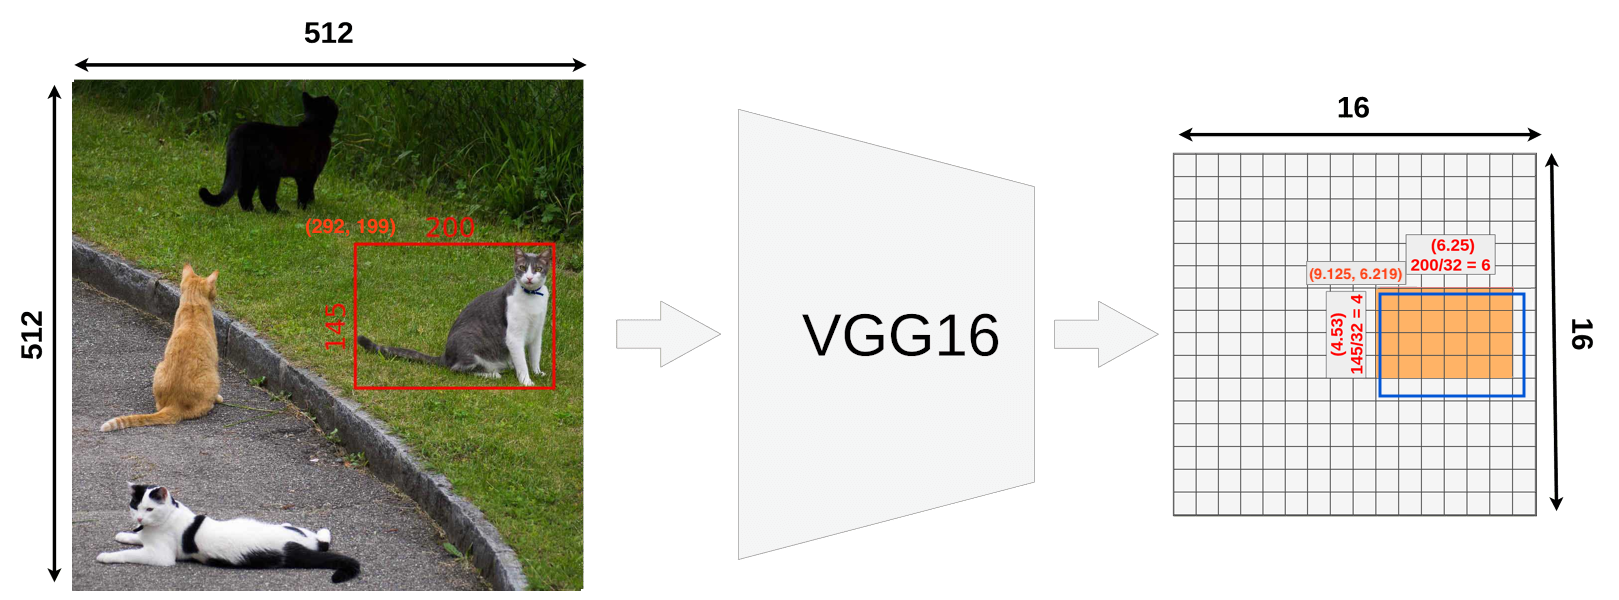
\includegraphics[width=6in]{figures/roi_projection_ex.png}
    \caption{RoI projection to feature map \cite{roi_pooling_problem}}
    \label{fig:roi_projection_ex}
\end{figure}

As an example, assume that we are processing an input image of $512 \times 512$ with VGG16, and the first fully connected layer expects $3 \times 3$ as input [Fig. \ref{fig:roi_projection_ex}]. Consider the input RoI with the top left corner coordinate of $(292, 199)$ and the size of $145 \times 200$. As mentioned earlier, VGG16 has a scale-down factor of $32$ from the input image to the feature map space. With this information, we can compute the corresponding coordinate and size of the input RoI in the feature map as follows:

Feature map RoI corner coordinate:
$$ \left( \floor{\frac{292}{32}}, \floor{\frac{199}{32}} \right) \ \ = \ \ \left( \floor{9.125}, \floor{6.21875} \right) \ \ = \ \ (9, 6) $$

Feature map RoI size: 
$$ \floor{\frac{200}{32}} \times \floor{\frac{145}{32}} \ \ = \ \ \floor{6.25} \times \floor{4.53125} \ \ = \ \ 6 \times 4 $$

\noindent When projecting to the feature map space, Fast R-CNN offsets and resizes the original projected RoI (shown as the blue rectangle in Fig. \ref{fig:roi_projection_ex}) to align perfectly with $n$ feature map pixels (shown as the orange area in Fig. \ref{fig:roi_projection_ex}), where $n$ is the number of feature map pixels that can fit entirely within the original projected RoI. As shown in Fig. \ref{fig:roi_projection_ex}, we lose some pixels data (the white part inside the blue rectangle) and have additional noise data (the orange part outside the blue rectangle). Consider the quantization of the conner's vertical position at 6.21875 to 6 in feature map space. When we factor in the scaling of 32 times, this means our projected RoI is shifted by $(6.21875 - 6) \times 32 = 7$ pixels vertically compared to the input RoI in the original image space. Similarly, the projected RoI is offset by 4 pixels horizontally, and the quantization process results in a loss of $(0.25 + 0.53125) \times 32 = 25$ pixels during projection.

\begin{figure}[!ht]
    \centering
    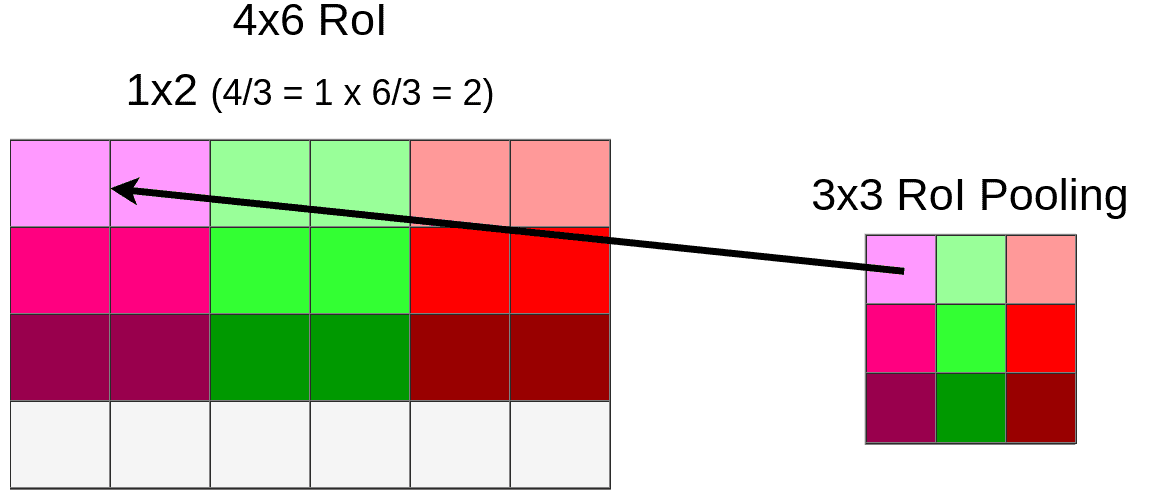
\includegraphics[width=4in]{figures/roi_pool_ex.png}
    \caption{The RoI feature grid is divided into RoI bins, as shown on the left. Performing max-pooling on each RoI bin results in a $3 \times 3$ output matrix, as shown on the right. Each cell in the input image represents a feature map pixel, and each RoI bin contains 2 pixels and has a unique color. Each cell in the output $3 \times 3$ matrix represents the highest feature map pixel out of all pixels in each corresponding RoI bin. The white cells on the left do not belong to any RoI bin and are not used in the RoI pooling process.\cite{roi_pooling_problem}}
    \label{fig:roi_pool_ex}
\end{figure}

After projecting and quantizing the input RoI, we obtain an RoI feature grid. In our example, this grid has dimensions of $6 \times 4$ and is located at position (9, 6). However, the next layer in our network requires inputs of size $3 \times 3$. To accommodate this, we divide the RoI feature grid into a grid of RoI bins, each with a size of $\frac{6}{3} \times \frac{4}{3} \approx 2 \times 1.3333$. Since these sizes are expressed in terms of pixel counts, we must quantize them to the nearest integer values, resulting in RoI bins of size $2 \times 1$. As shown in Fig. \ref{fig:roi_pool_ex}, this quantization results in the loss of information for the bottom row of pixels in the RoI feature grid, corresponding to a loss of $6 \times 32 = 192$ pixels in the input image space. In addition, the pooling operation can also cause small offsets in the position of the RoI bins, leading to further loss of information. Combined with every loss that happens in the RoIPool layer, the model has loss $192+25=217$ pixels. In addition, the RoI used for classification is offset by 7 pixels vertically and 4 pixels horizontally. While the loss of 217 pixels due to quantization and pooling may seem small compared to 29,000 pixels in the input RoI of size $200 \times 145$, thereby can be overlooked in the object detection task. However, as the goal of our study lies in the instance segmentation task, where the model outputs a mask containing every pixel belonging to the object, every pixel counts. Nonetheless, these losses in information and offset are for one input RoI. Due to the fact that object identification tasks typically detect multiple objects per image, the loss of information and offset caused by quantization may compromise the quality of the model. 

To address the quantization issue in the RoIPool layer, RoIAlign was proposed as a method for achieving size-independent downsampling without quantization. The RoIAlign is utilized with Mask R-CNN, an instance segmentation model that will be discussed in greater detail in Sec. \ref{sec:mask_rcnn}. Since Mask R-CNN is built on top of Faster R-CNN, which is also the subsequent significant improvement over the Fast R-CNN model, we will discuss the Faster R-CNN model in the following section. Faster R-CNN proposes the addition of the region proposal network (RPN) to resolve the bottleneck in object detection performance caused by object proposal runtime \cite{faster_rcnn_2015}. Instead of attempting to reduce the runtime of the object proposal algorithm, RPN's primary objective is to share computation with the object classification module, thereby allowing the object detection model to generate object proposals at no additional cost. We will further discuss the region proposal network (RPN) used in conjunction with Fast R-CNN to create Faster R-CNN in section \ref{sec:faster_rcnn}.